
%% bare_conf.tex
%% V1.3
%% 2007/01/11
%% by Michael Shell
%% See:
%% http://www.michaelshell.org/
%% for current contact information.
%%
%% This is a skeleton file demonstrating the use of IEEEtran.cls
%% (requires IEEEtran.cls version 1.7 or later) with an IEEE conference paper.
%%
%% Support sites:
%% http://www.michaelshell.org/tex/ieeetran/
%% http://www.ctan.org/tex-archive/macros/latex/contrib/IEEEtran/
%% and
%% http://www.ieee.org/

%%*************************************************************************
%% Legal Notice:
%% This code is offered as-is without any warranty either expressed or
%% implied; without even the implied warranty of MERCHANTABILITY or
%% FITNESS FOR A PARTICULAR PURPOSE! 
%% User assumes all risk.
%% In no event shall IEEE or any contributor to this code be liable for
%% any damages or losses, including, but not limited to, incidental,
%% consequential, or any other damages, resulting from the use or misuse
%% of any information contained here.
%%
%% All comments are the opinions of their respective authors and are not
%% necessarily endorsed by the IEEE.
%%
%% This work is distributed under the LaTeX Project Public License (LPPL)
%% ( http://www.latex-project.org/ ) version 1.3, and may be freely used,
%% distributed and modified. A copy of the LPPL, version 1.3, is included
%% in the base LaTeX documentation of all distributions of LaTeX released
%% 2003/12/01 or later.
%% Retain all contribution notices and credits.
%% ** Modified files should be clearly indicated as such, including  **
%% ** renaming them and changing author support contact information. **
%%
%% File list of work: IEEEtran.cls, IEEEtran_HOWTO.pdf, bare_adv.tex,
%%                    bare_conf.tex, bare_jrnl.tex, bare_jrnl_compsoc.tex
%%*************************************************************************

% *** Authors should verify (and, if needed, correct) their LaTeX system  ***
% *** with the testflow diagnostic prior to trusting their LaTeX platform ***
% *** with production work. IEEE's font choices can trigger bugs that do  ***
% *** not appear when using other class files.                            ***
% The testflow support page is at:
% http://www.michaelshell.org/tex/testflow/



% Note that the a4paper option is mainly intended so that authors in
% countries using A4 can easily print to A4 and see how their papers will
% look in print - the typesetting of the document will not typically be
% affected with changes in paper size (but the bottom and side margins will).
% Use the testflow package mentioned above to verify correct handling of
% both paper sizes by the user's LaTeX system.
%
% Also note that the "draftcls" or "draftclsnofoot", not "draft", option
% should be used if it is desired that the figures are to be displayed in
% draft mode.
%
\documentclass[10pt, conference, compsocconf]{IEEEtran}
% Add the compsocconf option for Computer Society conferences.
%
% If IEEEtran.cls has not been installed into the LaTeX system files,
% manually specify the path to it like:
% \documentclass[conference]{../sty/IEEEtran}





% Some very useful LaTeX packages include:
% (uncomment the ones you want to load)


% *** MISC UTILITY PACKAGES ***
%
%\usepackage{ifpdf}
% Heiko Oberdiek's ifpdf.sty is very useful if you need conditional
% compilation based on whether the output is pdf or dvi.
% usage:
% \ifpdf
%   % pdf code
% \else
%   % dvi code
% \fi
% The latest version of ifpdf.sty can be obtained from:
% http://www.ctan.org/tex-archive/macros/latex/contrib/oberdiek/
% Also, note that IEEEtran.cls V1.7 and later provides a builtin
% \ifCLASSINFOpdf conditional that works the same way.
% When switching from latex to pdflatex and vice-versa, the compiler may
% have to be run twice to clear warning/error messages.






% *** CITATION PACKAGES ***
%
%\usepackage{cite}
% cite.sty was written by Donald Arseneau
% V1.6 and later of IEEEtran pre-defines the format of the cite.sty package
% \cite{} output to follow that of IEEE. Loading the cite package will
% result in citation numbers being automatically sorted and properly
% "compressed/ranged". e.g., [1], [9], [2], [7], [5], [6] without using
% cite.sty will become [1], [2], [5]--[7], [9] using cite.sty. cite.sty's
% \cite will automatically add leading space, if needed. Use cite.sty's
% noadjust option (cite.sty V3.8 and later) if you want to turn this off.
% cite.sty is already installed on most LaTeX systems. Be sure and use
% version 4.0 (2003-05-27) and later if using hyperref.sty. cite.sty does
% not currently provide for hyperlinked citations.
% The latest version can be obtained at:
% http://www.ctan.org/tex-archive/macros/latex/contrib/cite/
% The documentation is contained in the cite.sty file itself.






% *** GRAPHICS RELATED PACKAGES ***
%
\ifCLASSINFOpdf
   \usepackage[pdftex]{graphicx}
  % declare the path(s) where your graphic files are
   \graphicspath{{./images/}}
  % and their extensions so you won't have to specify these with
  % every instance of \includegraphics
   \DeclareGraphicsExtensions{.pdf,.jpeg,.png}
\else
  % or other class option (dvipsone, dvipdf, if not using dvips). graphicx
  % will default to the driver specified in the system graphics.cfg if no
  % driver is specified.
  % \usepackage[dvips]{graphicx}
  % declare the path(s) where your graphic files are
  % \graphicspath{{../eps/}}
  % and their extensions so you won't have to specify these with
  % every instance of \includegraphics
  % \DeclareGraphicsExtensions{.eps}
\fi
% graphicx was written by David Carlisle and Sebastian Rahtz. It is
% required if you want graphics, photos, etc. graphicx.sty is already
% installed on most LaTeX systems. The latest version and documentation can
% be obtained at: 
% http://www.ctan.org/tex-archive/macros/latex/required/graphics/
% Another good source of documentation is "Using Imported Graphics in
% LaTeX2e" by Keith Reckdahl which can be found as epslatex.ps or
% epslatex.pdf at: http://www.ctan.org/tex-archive/info/
%
% latex, and pdflatex in dvi mode, support graphics in encapsulated
% postscript (.eps) format. pdflatex in pdf mode supports graphics
% in .pdf, .jpeg, .png and .mps (metapost) formats. Users should ensure
% that all non-photo figures use a vector format (.eps, .pdf, .mps) and
% not a bitmapped formats (.jpeg, .png). IEEE frowns on bitmapped formats
% which can result in "jaggedy"/blurry rendering of lines and letters as
% well as large increases in file sizes.
%
% You can find documentation about the pdfTeX application at:
% http://www.tug.org/applications/pdftex





% *** MATH PACKAGES ***
%
\usepackage[cmex10]{amsmath}
% A popular package from the American Mathematical Society that provides
% many useful and powerful commands for dealing with mathematics. If using
% it, be sure to load this package with the cmex10 option to ensure that
% only type 1 fonts will utilized at all point sizes. Without this option,
% it is possible that some math symbols, particularly those within
% footnotes, will be rendered in bitmap form which will result in a
% document that can not be IEEE Xplore compliant!
%
% Also, note that the amsmath package sets \interdisplaylinepenalty to 10000
% thus preventing page breaks from occurring within multiline equations. Use:
%\interdisplaylinepenalty=2500
% after loading amsmath to restore such page breaks as IEEEtran.cls normally
% does. amsmath.sty is already installed on most LaTeX systems. The latest
% version and documentation can be obtained at:
% http://www.ctan.org/tex-archive/macros/latex/required/amslatex/math/





% *** SPECIALIZED LIST PACKAGES ***
%
\usepackage{algorithm}
\usepackage{algorithmic}
% algorithmic.sty was written by Peter Williams and Rogerio Brito.
% This package provides an algorithmic environment fo describing algorithms.
% You can use the algorithmic environment in-text or within a figure
% environment to provide for a floating algorithm. Do NOT use the algorithm
% floating environment provided by algorithm.sty (by the same authors) or
% algorithm2e.sty (by Christophe Fiorio) as IEEE does not use dedicated
% algorithm float types and packages that provide these will not provide
% correct IEEE style captions. The latest version and documentation of
% algorithmic.sty can be obtained at:
% http://www.ctan.org/tex-archive/macros/latex/contrib/algorithms/
% There is also a support site at:
% http://algorithms.berlios.de/index.html
% Also of interest may be the (relatively newer and more customizable)
% algorithmicx.sty package by Szasz Janos:
% http://www.ctan.org/tex-archive/macros/latex/contrib/algorithmicx/




% *** ALIGNMENT PACKAGES ***
%
%\usepackage{array}
% Frank Mittelbach's and David Carlisle's array.sty patches and improves
% the standard LaTeX2e array and tabular environments to provide better
% appearance and additional user controls. As the default LaTeX2e table
% generation code is lacking to the point of almost being broken with
% respect to the quality of the end results, all users are strongly
% advised to use an enhanced (at the very least that provided by array.sty)
% set of table tools. array.sty is already installed on most systems. The
% latest version and documentation can be obtained at:
% http://www.ctan.org/tex-archive/macros/latex/required/tools/


%\usepackage{mdwmath}
%\usepackage{mdwtab}
% Also highly recommended is Mark Wooding's extremely powerful MDW tools,
% especially mdwmath.sty and mdwtab.sty which are used to format equations
% and tables, respectively. The MDWtools set is already installed on most
% LaTeX systems. The lastest version and documentation is available at:
% http://www.ctan.org/tex-archive/macros/latex/contrib/mdwtools/


% IEEEtran contains the IEEEeqnarray family of commands that can be used to
% generate multiline equations as well as matrices, tables, etc., of high
% quality.


%\usepackage{eqparbox}
% Also of notable interest is Scott Pakin's eqparbox package for creating
% (automatically sized) equal width boxes - aka "natural width parboxes".
% Available at:
% http://www.ctan.org/tex-archive/macros/latex/contrib/eqparbox/





% *** SUBFIGURE PACKAGES ***
%\usepackage[tight,footnotesize]{subfigure}
% subfigure.sty was written by Steven Douglas Cochran. This package makes it
% easy to put subfigures in your figures. e.g., "Figure 1a and 1b". For IEEE
% work, it is a good idea to load it with the tight package option to reduce
% the amount of white space around the subfigures. subfigure.sty is already
% installed on most LaTeX systems. The latest version and documentation can
% be obtained at:
% http://www.ctan.org/tex-archive/obsolete/macros/latex/contrib/subfigure/
% subfigure.sty has been superceeded by subfig.sty.



%\usepackage[caption=false]{caption}
%\usepackage[font=footnotesize]{subfig}
% subfig.sty, also written by Steven Douglas Cochran, is the modern
% replacement for subfigure.sty. However, subfig.sty requires and
% automatically loads Axel Sommerfeldt's caption.sty which will override
% IEEEtran.cls handling of captions and this will result in nonIEEE style
% figure/table captions. To prevent this problem, be sure and preload
% caption.sty with its "caption=false" package option. This is will preserve
% IEEEtran.cls handing of captions. Version 1.3 (2005/06/28) and later 
% (recommended due to many improvements over 1.2) of subfig.sty supports
% the caption=false option directly:
%\usepackage[caption=false,font=footnotesize]{subfig}
%
% The latest version and documentation can be obtained at:
% http://www.ctan.org/tex-archive/macros/latex/contrib/subfig/
% The latest version and documentation of caption.sty can be obtained at:
% http://www.ctan.org/tex-archive/macros/latex/contrib/caption/




% *** FLOAT PACKAGES ***
%
%\usepackage{fixltx2e}
% fixltx2e, the successor to the earlier fix2col.sty, was written by
% Frank Mittelbach and David Carlisle. This package corrects a few problems
% in the LaTeX2e kernel, the most notable of which is that in current
% LaTeX2e releases, the ordering of single and double column floats is not
% guaranteed to be preserved. Thus, an unpatched LaTeX2e can allow a
% single column figure to be placed prior to an earlier double column
% figure. The latest version and documentation can be found at:
% http://www.ctan.org/tex-archive/macros/latex/base/



%\usepackage{stfloats}
% stfloats.sty was written by Sigitas Tolusis. This package gives LaTeX2e
% the ability to do double column floats at the bottom of the page as well
% as the top. (e.g., "\begin{figure*}[!b]" is not normally possible in
% LaTeX2e). It also provides a command:
%\fnbelowfloat
% to enable the placement of footnotes below bottom floats (the standard
% LaTeX2e kernel puts them above bottom floats). This is an invasive package
% which rewrites many portions of the LaTeX2e float routines. It may not work
% with other packages that modify the LaTeX2e float routines. The latest
% version and documentation can be obtained at:
% http://www.ctan.org/tex-archive/macros/latex/contrib/sttools/
% Documentation is contained in the stfloats.sty comments as well as in the
% presfull.pdf file. Do not use the stfloats baselinefloat ability as IEEE
% does not allow \baselineskip to stretch. Authors submitting work to the
% IEEE should note that IEEE rarely uses double column equations and
% that authors should try to avoid such use. Do not be tempted to use the
% cuted.sty or midfloat.sty packages (also by Sigitas Tolusis) as IEEE does
% not format its papers in such ways.





% *** PDF, URL AND HYPERLINK PACKAGES ***
%
%\usepackage{url}
% url.sty was written by Donald Arseneau. It provides better support for
% handling and breaking URLs. url.sty is already installed on most LaTeX
% systems. The latest version can be obtained at:
% http://www.ctan.org/tex-archive/macros/latex/contrib/misc/
% Read the url.sty source comments for usage information. Basically,
% \url{my_url_here}.





% *** Do not adjust lengths that control margins, column widths, etc. ***
% *** Do not use packages that alter fonts (such as pslatex).         ***
% There should be no need to do such things with IEEEtran.cls V1.6 and later.
% (Unless specifically asked to do so by the journal or conference you plan
% to submit to, of course. )


% correct bad hyphenation here
\hyphenation{op-tical net-works semi-conduc-tor}


\begin{document}
% use linebreaks \\ within to get better formatting as desired
\title{Parallel Feature Extraction and Tracking for 3D Vortical Data (TBD)}

% author names and affiliations
% use a multiple column layout for up to two different
% affiliations

\author{\IEEEauthorblockN{Authors Name/s per 1st Affiliation (Author)}
\IEEEauthorblockA{line 1 (of Affiliation): dept. name of organization\\
line 2: name of organization, acronyms acceptable\\
line 3: City, Country\\
line 4: Email: name@xyz.com}
\and
\IEEEauthorblockN{Authors Name/s per 2nd Affiliation (Author)}
\IEEEauthorblockA{line 1 (of Affiliation): dept. name of organization\\
line 2: name of organization, acronyms acceptable\\
line 3: City, Country\\
line 4: Email: name@xyz.com}
}

% make the title area
\maketitle


\begin{abstract}
Large-scale time-varying volumetric data set can take terabytes to petabytes of memory to process. One promising approach is to process the data in parallel, extracting features of interest and analyze only those features. This requires memory space that is several orders of magnitude smaller. However, extracting volumetric features in parallel is a non-trivial task as features might span over multiple processors, and partial features are visible only within their own processor. In this paper, we discuss how to generate and maintain connectivity information of features reside in different processors. Based on this connectivity information, partial features can be integrated, which makes possible for the large-scale feature extraction and tracking in parallel. We demonstrate the effectiveness and scalability of our approaches by apply it to two volumetric flow data sets, and compare the pros and cons of each approach.
\end{abstract}

\begin{IEEEkeywords}
feature tracking; parallel graph;
\end{IEEEkeywords}

% For peer review papers, you can put extra information on the cover
% page as needed:
% \ifCLASSOPTIONpeerreview
% \begin{center} \bfseries EDICS Category: 3-BBND \end{center}
% \fi
%
% For peerreview papers, this IEEEtran command inserts a page break and
% creates the second title. It will be ignored for other modes.
\IEEEpeerreviewmaketitle

\section{Introduction}
% no \IEEEPARstart
The increasing computational power and accessibility to supercomputers have brought scientists the capability to simulate physical phenomena of unprecedented complexity at high spatial and temporal resolution. However, these large-scale time-varying data sets can take gigabyte or even terabytes of space to preserve. One promising solution to the problem is to introduce feature extraction and tracking techniques. Instead of duplicating raw data along the exploring process, dealing with features of interest requires memory space that is several orders of magnitude smaller than the raw data would take.
However, extracting and tracking features in distributed vortical datasets is a non-trivial task. Existing researches on feature-based data visualization have been done mostly focusing on decomposing features using quantitative measures such as size, location, shape or topology information, etc. These measures cannot be applied to distribute volume data directly since vortical features are consist of certain amount of voxels and are very likely to span over blocks as they evolve over time. Therefore existing quantitative measures of partial data scattered in different data blocks cannot be used to describe an integrated feature, unless the distribution of partial features can be obtained beforehand. 

To obtain the feature distribution, a connectivity map of each feature should be generated and maintained. In this paper, we proposed an approach for creating and maintaining feature residual, as well as connectivity information utilizing parallel graphs. Comparing to previous approaches, which generates and maintains the global features information in a single host node, our approach can be done locally that only involves residual data blocks of target features. This requires least communication overhead and avoids the potential bottleneck on the host node. We demonstrate the effectiveness of this method with three vortical flow datasets and the scalability of our system in a distributed environment.

% You must have at least 2 lines in the paragraph with the drop letter
% (should never be an issue)

\section{Related Work}
Extraction and tracking are two closely related problems in feature-based visualization. Although many feature tracking algorithms have been introduced, most of them extract features from single time steps and then try to associate them between consecutive time steps. Silver and Wang [26] considered threshold connected components as their features, and tracked overlapped features between successive time steps by calculating their differences. Octree was employed in their method to speed up the performance and the criteria they used were domain dependent. Reinders et al. [24] introduced a prediction verification tracking technique that calculates a prediction by linear extrapolation based on the previous feature path, an candidate will be added to the path if it corresponds to that prediction. Ji and Shen [17] introduced a method to track local features from time-varying data by using higher-dimensional isosurfacing. They also used a global optimization correspondence algorithm to improve the robustness of feature tracking [16]. Caban et al. [3] estimated  a tracking window and then tried to find the best match between that window and different sub-volumes of subsequence frames by comparing their distance of textural properties.  Also, Bremer et al. [1] described two topological feature tracking methods, one employs Jacobi sets to track critical points while another uses distance measures on graphs to track channel structures. 

Most of the above methods extract features from each time step independently and then apply the correspondence calculation. This could be very slow especially when the size of dataset becomes large. Muelder and Ma [19] introduced a prediction-correction approach that first predicts feature region based on the centroid location of previous time steps, then correcting the predicted region by adjusting the surface boundaries via region growing and shrinking. This approach is appealing because of its computing efficiency and the reliability in an interactive system.

From the parallel processing side of perspective, most of the existing feature extraction and tracking approaches rely on some form of global feature information, while in distributed environment must be communicated among processors to obtain. Chen and Silver [] introduced a two stage partial-merge strategy, exchanging local connectivity information using Binary-tree merge, then a visualization server correlate local data to create a global data. This approach is not scalable since half of the processors will become idle after each merge. It is also unclear that how the visualization server can efficiently collect local connectivity information from non-server processor, since gathering operation is typically very expensive given a large number of processors. 

The approach proposed in this paper follows a different paradigm. Instead of sending local connective information back to the host, the local connectivity information are computed and preserved only in nodes where correspondent feature resides in. There is no global connectivity information preserved in the host node and it only acts as the interface from where the criterion of feature of interest is broadcast. By doing this, the computation of merging local connectivity information is distributed to those non-host nodes and hence effectively reduces the potential communication bottleneck on the host node. What's more, there's no need to set a barrier and wait before all connectivity information was send back to the host and thus if there exists features that span over a large number of nodes but was not selected by the user, the potentially long computation time for these features will not block the whole process. This makes it ideal for an interactive system, where users can select the feature of interest and instantly receive the visual feedback as the feature evolves.

\textbf{[TODO] Add related work for parallel graph algorithms and data structures. (half page)}

\section{Algorithm Design}
Though features can be extracted within individual processors using the aforementioned methods, they might also span over multiple data blocks, which is unavoidable as the number of processors increases. To perform feature extraction and tracking over a distributed volume data set, information like how partial features are located and connected should be recorded and maintained. Feature descriptors such as size, curvature or velocity of partial features are not shared among processors, thus connectivity information makes it possible to gather from each part of the feature resides in different processors these descriptions such that feature tracking or and similarity test could be achieved. 

However, maintaining such connectivity information requires data exchange among different processors and hence will introduce extra communication cost. To design a proper communication schema for better performance and scalability, the following three factors should be carefully considered:

\begin{enumerate}
\item How many communications are required to complete the connectivity graph;
\item How many processors will be involved in one communication;
\item How much data will be sent and received in one communication.
\end{enumerate}

In the following sections, we will give a detailed description on how to create and maintain such connectivity information using an undirected unweighted graph to achieve minimum cost over the above three factors.

\subsection{Feature Extraction}
Feature extraction is a process that first detects features, then calculates quantitative attributes describing its characteristics. In general, features can be any interesting pattern, structure, or object that are considered relevant for investigation. In our application, features are defined as the collection of voxices that are located within certain isosurface. Such volumetric feature could be extracted by common techniques such as region growing, geometry or topology based clustering, or other domain specific algorithms as described in [] [] [] []. 

In our work, a standard region-growing algorithm [14] is used for partitioning the original volume data into an initial set of features. This can be done by first spreading a set of seeding points inside the volume, and then clustering voxices into separate regions, each regarded as a single feature. Usually, scientists prefer to focus on features that are meaningful as dictated by their underlying research goal. Potential features detected by the region-growing algorithm, however, are often cluttered and relatively coarse, which might be far from expected. On the other hand, reducing the number of tracked features makes sense from the perspective of computational expense. Therefore, after the potential features set was generated, an iterative process of refinement could be applied to refine the result. 

Existing research [27] has detailed the applicability and performance of context-based 3D shape descriptors and their corresponding retrieval methods. Based on the discussion in this work, we can characterize the interactive refinement process as primarily concerned with those computationally efficient yet with significant discriminating deformation robust descriptors, such as size, location, or skeletal curvature. After specific features have been extracted from a single time step, their evolution can be tracked over time using a prediction-correction approach. The prediction of features' region in space can be made based on the location of features reside in consecutive time steps. Once prediction is made, the actual region could be obtained by adjusting the surface of the predicted region: first shrink the edge surface points to obtain the mutual region between consecutive time steps, then use of a technique based on region-growing to obtain the actual region.

This prediction-correction approach was proved effective and efficient for single processor based feature tracking [32]. However, as the size of the volume data grows such that the original data cannot fit into one processor, a cluster of multiple processors need to be used to process the data in parallel. One challenge to parallelize the aforementioned approach lies in that, since volumetric features may span over multiple processors, the global feature descriptions could not be obtained unless they can be shared and merged in a efficient way, as partial features reside in different nodes will be operated independently. 

An intuitive way of exchanging such feature information is to first, find how features are connected when they span over multiple processors, and then merge feature descriptions according to the connectivity information.

\subsection{Creating Partial connectivity graph}
If we try to partition a large volumetric dataset using a regular processor grid, it is very likely that some of the features will be cut off on the boundary surface of its residing block. For these multinational features, the cross-sectional area on the block boundary surface should match. Leveraging this property, we could connect separate parts of a feature resides in adjacent data blocks by comparing their sectional area on the correspondent boundary surface. 

Since data is distributed, vortices in adjacent blocks are invisible to the current processor. Though exchanging all voxices on the sectional area would be sufficient for finding all possible matches, we choose to exchange more abstract data, e.g. the min-max coordinate of and the geometric centroid of the cross-sectional area to reduce the amount of data being sent over the network. The min-max coordinates are not optional because they ensure correct connectivity for some special cases where one cross-sectional area is surrounded by another concave or hollow area whose centroid happen to be the same, as depicted in figure 1.

\begin{figure}[htpb]
\centering
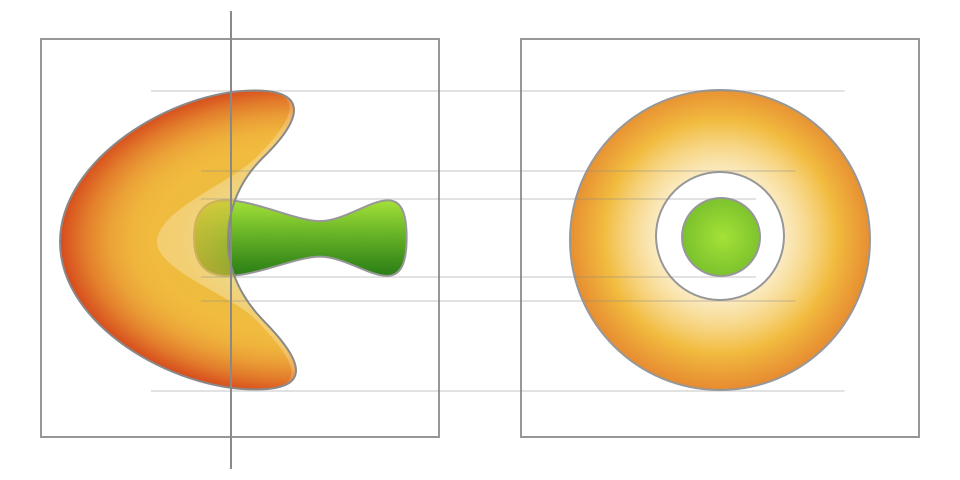
\includegraphics[width=2.5in]{figure1@2x.png}
\caption{A special case where two features share a same centroid}
\end{figure}

A voxel-width "ghost surface" that stores boundary surface belonging to neighboring blocks might help to achieve voxel-wise matching for partial features. However, for non-post-processing situation where data set are not pre-determined, maintaining such "ghost surface" requires frequent inter-process communication and is considered expensive for data generated in real-time. Instead, a ±1 voxel tolerance was given in our work when trying to match two geometric centroids on the boundary surfaces. That is, if the neighboring centroid is within the eight direct neighbor of the domestic centroid, they are considered a match and the two separated parts were belong to the same feature.

The creation of partial connectivity graph will not introduce extra computational cost as it could be done along with the region growing process. A new edge is appended to the existing graph when a local feature touches the block boundary, taking the ID of the target block that shares a same boundary surface as the ending vertex, as well as the global index of the centroids point as edge value.

The detailed algorithm of creating local partial connectivity graph is given in Algorithm 1.
%------------------------------------------------
\begin{algorithm}
\caption{Creating Partial Connectivity Graph}
\begin{algorithmic}[1]
\STATE $edgeList \leftarrow new List()$
\STATE $featureList \leftarrow new List()$
\IF{Current time step $t = t0$}
	\STATE // Initialize random seeding points
	\STATE $seedList \leftarrow randomVortices()$
	\FOR {each $seed$ in $seedList$}
		\STATE $feture \leftarrow expendRegion()$
		\STATE append $feture$ to $featureList$
	\ENDFOR	
\ELSE
	\FOR {each $feture$ in $featureList$}
		\STATE $feture \leftarrow predictRegion()$
		\STATE $feture \leftarrow adjustRegion()$	
		
		\STATE $start \leftarrow$ current processor ID
		\STATE $end \leftarrow$ target neighboring processor ID
		\STATE $min,max \leftarrow$ min-max boundary coordinate
		\STATE $index \leftarrow$ global voxel index of centroid
		\STATE Edge $e = Edge(start, end, min, max, index)$
		\STATE append $e$ to $edgeList$
	\ENDFOR
\ENDIF
\end{algorithmic}
\begin{algorithmic} \STATE \end{algorithmic}	% line separator
\begin{algorithmic}[1]
\STATE $adjustRegion()$
	\IF{Voxel $v$ on boundary surface}
		\STATE $updateMixMaxBoundary()$
		\STATE $updateBoundaryCentroid()$
	\ENDIF
\end{algorithmic}
\end{algorithm}
%------------------------------------------------

// TODO (put to result, performance analyze)
Memory cost, each feature on boundary will use two INTs, 1 as global centroids coordinate, the other as target node number. even if there's 1000 features on the boundary, it won’t cost more than 1000 * 5 * 4 = 20mb to store this graph, neglectable compare to the volume data itself. (But kind of large if used for communication)

\subsection{Creating Global Connectivity Graph}
\subsubsection{The naive solution}
To obtain the global description of a partitioned feature, local connectivity graph need to be merged with those derived from their neighboring processors, after they were individually created. A naive approach to gather local connectivity graphs is to send all edges sharing the same ending vertex to that target processor, and to merge edges sent from neighboring processor. Two edges are merged if they suffice the following three condition:

\begin{enumerate}
\item The starting and ending vertices are reversely matched;
\item The min-max boundary coordinate do match;
\item Edge centroid located within direct neighbors.
\end{enumerate}

Recall that the starting vertex of an edge represents the current processor ID and ending vertex the ID of target processor, whose data block is adjacent to the one that reside in the current processor, and the edge value is encoded by the global coordinate of the geometric centroid and min-max boundary on the shared boundary surface and. If two edges match to each other, the two partial features must share a same boundary surface with the same centroid and bounding region. In other word, these two partial features were cut off when partitioning the original data set, and should be considered the same feature sharing a same feature ID.

The detailed algorithm of merging matched edges (henceforth referred to as REDUCE) is given in Algorithm 2.
%------------------------------------------------
\begin{algorithm}
\caption{REDUCE: Merging Matched Edges}
\begin{algorithmic}[1]
\REQUIRE $localEdges$, $recievedEdges$
\FOR {each $ei$ in $localEdges$}
	\FOR {each $ej$ in $recievedEdges$}
		\IF{$ei.start$ = $ej.end$ and $ej.start$ = $ei.end$ \textbf{and}
			$ei.min$ = $ej.min$ and $ei.max$ = $ej.max $ \textbf{and}
			$ei.centroid \approx ej.centroid$}
			\IF {$ei.id < ej.id$}
				\STATE $ej.id \leftarrow ei.id$
			\ELSE
				\STATE $ei.id \leftarrow ej.id$
			\ENDIF
		\ENDIF
	\ENDFOR	
\ENDFOR	
\end{algorithmic}
\end{algorithm}
%------------------------------------------------

This naive solution may work for data set with small sized features, however, if we consider the case that there exists a long curly feature inside the volume and was partitioned evenly over the grid. In order to gather and merge the whole feature, the processors need to talk to its neighbor and spread the edge exchange operation one by one like that in the "telephone" game. This takes O(N) times communication to connect a single feature, where N is the number of total number of processors in the grid. And consequently O(nf * N) times communication, where nf is the number of features, for all the features within one time step. Also, since one processor has no idea if it will receive any edges from its adjacent processors, it is hard to schedule the communication process.

\subsubsection{The centralized approach}
A possible solution to reduce the number of times required for merging all edges is to employ the master-slave hierarchy by introducing a separate host processor. When the feature extraction process is done, local connectivity graphs with edges representing how many features have touched the block boundary as well as where they are located on the surface within each individual processor will be gathered to the host processor. After this \textit{Gather} operation is done, i.e. host processor has collected all local connectivity graphs, the REDUCE operation starts to merge edges from each partial graph to a single global connectivity graph.

The merit of this centralized approach lies in that it requires inter-processor communication only once. What is more, a global graph of feature information could be preserved in the host processor, which makes it easy for the host to response directly without pulling information from slave processors a second time. However the drawback of this approach is also obvious. Since all partial connectivity graphs preserved in each processor will be sent to a single processor, there exists potential bottlenecks, both communication and computational, on the host processor.

\subsubsection{The decentralized approach}
A better solution is to decentralize from REDUCE on a single host processor to all processors that are available. After the feature extraction process is done and so does the creation of local connectivity graphs, an \textit{Allgather} process starts to exchanging all local connectivity graphs within each processor to all the others. Each processor will first collect a full copy of all local connectivity graphs followed by the same REDUCE process to merge the edges into a single concise connectivity graph. 

\begin{figure}[htpb]
\centering
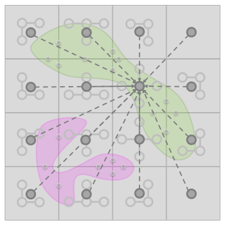
\includegraphics[width=1.5in]{figure3.png}
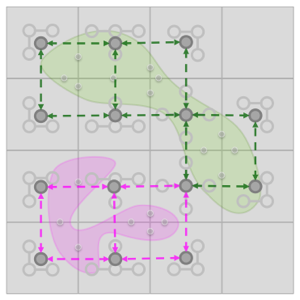
\includegraphics[width=1.5in]{figure4.png}
\caption{Left: each processor gather partial graphs from all the other processors; Right, A special case where two features share a same centroid}
\end{figure}

Though the "redundant" host processor is no more required when applying for computation resources, this approach does not actually solve the bottleneck problem since now every processor is now acting like a host since they still need to gather all partial graphs and try merging them together. For real world data set, however, it is rarely the case that a single feature will span over every processor. In other word, it is unnecessary to gather edges of feature that are not reside in current processor. To reduce the redundant communications with every other processor in the grid, the decentralized approach could be further improved such that we only consider those processors that are directly adjacent to the current one. That is, each processor only talks to its direct neighbors and shares information with them regardless what is happening outside. 

For a regularly partitioned volumetric data set, there are only 6 direct neighbors for each processor (for processor on the "edge" of the grid there are even less). Instead of gathering connectivity information from all processors in the grid, only graphs reside in neighboring processors will be gathered. This could be considered as a higher level of region growing, starting from one seeding processor and then grows from its adjacent processors, exchanging and merging connectivity information in a bread-first fashion until all cross-boundary features are connected. 

The detailed scheduling algorithm is depicted in Algorithm 3. 
%------------------------------------------------
\begin{algorithm}
\caption{Processor Level Region Growing}
\begin{algorithmic}[1]
\REQUIRE $adjacentProcessors$, $localEdges$
\STATE $toSend, toRecv \leftarrow true$	// init scheduling flags
\STATE $\delta \leftarrow localEdges$	// init data to be sent
\WHILE {$toSend$ = $true$ or $toRecv$ = $true$}
	\STATE $target \leftarrow toRecv$ = $true$ ? $myRank$ : null
	\STATE $procsToSync \leftarrow Allgather(target)$
	\FOR {each $proc$ in $procsToSync$}
		\IF {$toSend$ = $true$}
			\STATE send $\delta$ to $proc$
		\ENDIF
		\IF {$toRecv$ = $true$}
			\STATE receive $\delta\prime$ from $proc$
		\ENDIF
	\ENDFOR
	\STATE $toSend \leftarrow procsToSync$ is empty ? $false$ : $true$
	\STATE $toRecv \leftarrow false$
	\STATE $localEdges \leftarrow Reduce(localEdges, \delta\prime)$
\ENDWHILE
\end{algorithmic}
\begin{algorithmic} \STATE \end{algorithmic}	% line separator
\begin{algorithmic}[1]
\STATE $Reduce(localEdges, \delta\prime)$
	\FOR {each $edge$ in $\delta\prime$}
		\IF {$edge$ is new}
			\STATE add $edge$ to $\delta$
			\STATE $toRecv \leftarrow true$
		\ENDIF
	\ENDFOR	
\end{algorithmic}
\end{algorithm}
%------------------------------------------------

For the worst case that a feature spans over all of the processors, it takes O(C∛(|N|)) time to finish the search for connected processors, much faster than the previous O(N) time for all gathering among all processors.

\subsubsection{The hybrid approach}
We can still take a step further to optimize the aforementioned decentralized approach. As volume data evolves over time, the internal features may vary but should not change drastically in size and shape nor location if the time interval for sampling is short enough. Thus we can apply the prediction-correction approach to further reduce the number of times required to complete the connectivity graph. 

Every time (say, ti) when the global connectivity graph is completed, new local communicators will be updated for the next time step (ti+1), with the union of processors that share a same edge with the current processor, as shown in figure x. Edges from these processors are required to complete the global connectivity graph anyway, no matter which approach is used. Hence, for these must-involve processors, we apply the Decentralize-I approach, allowing the minimum one-time synchronization to finish gathering all edges necessary for updating the connectivity graph based on the graph created at previous time step (t). Then, the processor-level region growing explained in 3.3.3 is applied to extend the "boundary" of processes, obtaining newly connected processors caused by the evolution of the original volume. Beside, only those edges that are changed and not synchronized will be sent. This makes sure we keep the amount of data being sent over network to the minimum necessity.
The detail algorithm of the hybrid approach is given in Table x.

\section{Application}

\subsection{Feature selection and refinement}
Since the feature extraction are done independently within each PE, one of the potential function need to be addressed is that how do they know if their adjacent processor was has the feature to be highlighted and whether it has the other part of the features. Intuitively, sending a message to the adjacent PE whenever a feature was detected touching the surface boundary can do this. But if the target feature spans over multiple PEs, this sending/receiving procedure would take several rounds to end. This is potentially a big problem when the PE/Volume ratio is relatively high such that each feature spans over a lot of PEs. Another problem is that, if a PEs has two selected features whose connectivity info arrives in different rounds, it requestes to calculate twice, which again, will become a problem when PE/Volume ratio is large.

By introducing the global connectivity graph in our approach, whenever part of the feature was selected, the unique feature id will be sent back to host processor and then broadcast to all PEs contains it, and only in one rounds, the selection can be finished.

Based on the coordinate user specified or clicked on the volume rendering result, the residual processor as well as the feature, if the point was included by, could be obtains. Then the host processor can simply broadcast the selected feature id to all those processors who has the partial feature such that they can be highlighted.


\subsection{Feature tracking}
Before you begin to format your paper, first write and save the content as a separate text file. Keep your text and graphic files separate until after the text has been formatted and styled. Do not use hard tabs, and limit use of hard returns to only one return at the end of a paragraph. Do not add any kind of pagination anywhere in the paper. Do not number text heads-the template will do that for you.

Finally, complete content and organizational editing before formatting. Please take note of the following items when proofreading spelling and grammar:

\section{Result}
\subsection{Performance Result}
\subsection{Visualization Result}

\section{Conclusion}
In this paper, we proposed a decentralized approach that all feature connectivity information are created and preserved in distributed processors. Traditional approaches perform connectivity test on each processor and subsequently correspond them in a host processor after gathering all or partially merged connectivity information. Our approach does not follow this paradigm. Rather, instead of sending local connectivity information back to the host, they are computed and preserved only in processors where correspondent feature resides in. There is no copy of the global feature information preserved in the host processors and it only acts as the interface from where the criterion of feature of interest is broadcast. By doing this the computation of merging local connectivity information is distributed to the non-host s and it effectively reduces the potential communication bottleneck on the host processor. What's more, there's no need to set a barrier and wait before all connectivity information was send back to the host, thus if one of the features spans over a large number of processors but was not selected by the user, the potentially long computation time for this feature will not be considered. This makes it ideal for an interactive system, where users can select the feature of interest and instantly receive the visual feedback as the feature evolves.

% An example of a floating table. Note that, for IEEE style tables, the 
% \caption command should come BEFORE the table. Table text will default to
% \footnotesize as IEEE normally uses this smaller font for tables.
% The \label must come after \caption as always.
%
%\begin{table}[!t]
% increase table row spacing, adjust to taste
%\renewcommand{\arraystretch}{1.3}
% if using array.sty, it might be a good idea to tweak the value of
% \extrarowheight as needed to properly center the text within the cells
%\caption{An Example of a Table}
%\label{table_example}
%\centering
% Some packages, such as MDW tools, offer better commands for making tables
% than the plain LaTeX2e tabular which is used here.
%\begin{tabular}{|c||c|}
%\hline
%One & Two\\
%\hline
%Three & Four\\
%\hline
%\end{tabular}
%\end{table}


% Note that IEEE does not put floats in the very first column - or typically
% anywhere on the first page for that matter. Also, in-text middle ("here")
% positioning is not used. Most IEEE journals/conferences use top floats
% exclusively. Note that, LaTeX2e, unlike IEEE journals/conferences, places
% footnotes above bottom floats. This can be corrected via the \fnbelowfloat
% command of the stfloats package.


% use section* for acknowledgement
\section*{Acknowledgment}


The authors would like to thank...
more thanks here


% trigger a \newpage just before the given reference
% number - used to balance the columns on the last page
% adjust value as needed - may need to be readjusted if
% the document is modified later
%\IEEEtriggeratref{8}
% The "triggered" command can be changed if desired:
%\IEEEtriggercmd{\enlargethispage{-5in}}

% references section

% can use a bibliography generated by BibTeX as a .bbl file
% BibTeX documentation can be easily obtained at:
% http://www.ctan.org/tex-archive/biblio/bibtex/contrib/doc/
% The IEEEtran BibTeX style support page is at:
% http://www.michaelshell.org/tex/ieeetran/bibtex/
%\bibliographystyle{IEEEtran}
% argument is your BibTeX string definitions and bibliography database(s)
%\bibliography{IEEEabrv,../bib/paper}
%
% <OR> manually copy in the resultant .bbl file
% set second argument of \begin to the number of references
% (used to reserve space for the reference number labels box)
\begin{thebibliography}{1}

\bibitem{}
P.-T. Bremer, E.M. Bringa,M. A. Duchaineau, A. G. Gyulassy, D. Laney, A. Mascarenhas, and V. Pascucci. Topological feature extraction and tracking. Journal of Physics: Conference Series, 78(1):7–12, 2007.

\bibitem{}
X. T. C. Garth. Topology- and feature-based flow visualization: Methods and applications. SIAM Conference on Geometric Design and Computing, 2005.

\bibitem{}
J. Caban, A. Joshi, and P. Rheingans. Texture-based feature tracking for effective time-varying data visualization. IEEE Transactions on Visualization and Computer Graphics, 13(6):1472–1479, 2007.

\bibitem{}
N. D. Cornea, D. Silver, and P. Min. Curve-skeleton applications. In Proceedings of the IEEE Visualization Conference, pages 13–21, 2005.

\bibitem{}
N. D. Cornea, D. Silver, and P. Min. Curve-skeleton properties, applications, and algorithms. IEEE Transactions on Visualization and Computer Graphics, 13(3):530–548, 2007.

\bibitem{}
J. Ebling and G. Scheuermann. Clifford convolution and pattern matching on vector fields. In VIS ’03: Proceedings of the 14th IEEE Visualization 2003 (VIS’03), page 26, 2003.

\bibitem{}
J. Ebling and G. Scheuermann. Clifford fourier transform on vector fields. IEEE Transactions on Visualization and Computer Graphics, 11(4):469–479, 2005.

\bibitem{}
J. Ebling and G. Scheuermann. Clifford Convolution and Pattern Matching on Irregular Grids. Springer Berlin Heidelberg, 2006.

\bibitem{}
H. Hauser, H. Hagen, and H. Theisel. Topology-based Methods in Visualization. Springer Publishing Company, Incorporated, 2007.

\bibitem{}
H.-C. Hege, K. Polthier, and G. Scheuermann. Topology-Based Methods in Visualization II. Springer Publishing Company, Incorporated, 2008.

\bibitem{}
E. Heiberg, T. Ebbers, L. Wigstr, and M. Karlsson. Three-dimensional flow characterization using vector pattern matching. IEEE Transactions on Visualization and Computer Graphics, 9:313–319, 2003.

\bibitem{}
J. L. Helman and L. Hesselink. Representation and display of vector field topology in fluid flow data sets. Computer, 22(8):27–36, 1989.

\bibitem{}
H. Helwig. Visual analysis of deferential information. In Proceedings of the International Conference of Applied Mathematics, 2006.

\bibitem{}
R. Huang and K.-L. Ma. Rgvis: Region growing based techniques for volume visualization. In Proceedings of Pacific Graphics 2003 Conference, pages 355–363, October 2003.

\bibitem{}
J. Jeong and F. Hussain. On the identification of a vortex. Journal of Fluid Mechanics, pages 69–94, June 1995.

\bibitem{}
G. Ji and H.-W. Shen. Feature tracking using earth mover’s distance and global optimization. In Pacific Graphics, 2006.

\bibitem{}
G. Ji, H.-W. Shen, and R. Wenger. Volume tracking using higher dimensional isosurfacing. In Proceedings of the IEEE Visualization Conference, pages 209–216, 2003.

\bibitem{}
M. Jiang, R. Machiraju, and D. Thompson. Detection and visualization of vortices. In The Visualization Handbook, pages 295–309, 2005.

\bibitem{}
C. Muelder and K.-L. Ma. Interactive feature extraction and tracking by utilizing region coherency. In Proceedings of IEEE Pacific Visualization 2009 Symposium, April 2009.

\bibitem{}
K. Pal´agyi and A. Kuba. A parallel 3d 12-subiteration thinning algorithm. Graph. Models Image Process., 61(4):199–221, 1999.

\bibitem{}
S. W. Park, B. Budge, L. Linsen, B. Hamann, and K. I. Joy. Multidimensional transfer functions for interactive 3d flow visualization. In PG ’04: Proceedings of the Computer Graphics and Applications, 12th Pacific Conference, pages 177–185, 2004.

\bibitem{}
A. Pobitzer, R. Peikert, R. Fuchs, B. Schindler, A. Kuhn, H. Theisel, K. Matkovic, and H. Hauser. On the way towards topology-based visualization of unsteady flow – the state of the art. In accepted for Eurographics 2010 - State of the Art Reports, April 2010.

\bibitem{}
F. H. Post, B. Vrolijk, H. Hauser, R. S. Laramee, and H. Doleisch. The state of the art in flow visualization: Feature extraction and tracking. Comput. Graph. Forum, 22(4):775–792, 2003.

\bibitem{}
K. F. Reinders, K. Frederik, and J. Reinders. Feature-Based Visualization of Time-Dependent Data. PhD thesis, 2001. 

\bibitem{}
M. Schlemmer, M. Heringer, F. Morr, I. Hotz, M. Hering-Bertram, C. Garth, W. Kollmann, B. Hamann, and H. Hagen. Moment invariants for the analysis of 2d flow fields. IEEE Transactions on Visualization and Computer Graphics, 13(6):1743–1750, 2007.

\bibitem{}
D. Silver and X. Wang. Tracking and visualizing turbulent 3d features. IEEE Transactions on Visualization and Computer Graphics, 3(2):129– 141, 1997.

\bibitem{}
J. W. H. Tangelder and R. C. Veltkamp. A survey of content based 3d shape retrieval methods. In SMI ’04: Proceedings of the Shape Modeling International 2004, pages 145–156, 2004.

\bibitem{}
O. Amoros, S. Escalera, and A. uig. Adaboost GPU-based Classifier for Direct Volume Rendering. GRAPPSciTePress (2011), p. 215-219.

\bibitem{}
The State of the Art of Flow Visualization: Feature Extraction and Tracking. 

\end{thebibliography}

% that's all folks
\end{document}